\section{Model \#2: fixed planets and primaries, varying secondaries}
\label{sec:model_2}

The main use of our binary-twin model was to help develop intuition.
Gradually introducing complexity, we now let the light ratio $\gamma_R = 
L_2/L_1$ vary across the binary population.
It does so because the underlying mass ratio $q=M_2/M_1$ varies.
We keep the primary mass fixed as $M_1$, which is also the mass of all single 
stars.

We parametrize the distribution of binary mass ratios in a volume-limited 
sample as a power law: $p(q)\propto q^\beta$.
For binaries with solar-type primaries\footnote{
Duchene and Kraus (2013), fitting all the multiple systems of Raghavan et al. 
(2010)'s Fig 16, find $\beta = 0.28\pm0.05$ for $0.7<M_\star/M_\odot<1.3$.
Examining only the binary systems of Rhagavan et al 2010, Fig 16, the 
distribution seems roughly uniform, $\beta \approx 0$, except for a claimed 
excess of twin binaries with $q\approx 1$, and a deficiency of $q<0.1$ 
stellar companions.
}, $\beta$ is probably between 0 and 0.3.
Since we assume stars are a one-parameter family, $R \propto M \propto 
L^{1/\alpha}$, a drawn value of $q$ determines everything about a secondary.

The rate density in this model, $\Gamma(\vec{x})$, is the sum over system 
types of $w_i \Lambda_i p_i(\vec{x})$:
\begin{equation}
\Gamma(\vec{x})
=
\delta^4(r_p,R_\star,a_p,P_p)(w_0 \Lambda_0 + w_1 \Lambda_1)
+ w_2 \Lambda_2 \delta^3(r_p, P_p, a_p) p_2(q),
\label{eq:model2_rate_density}
\end{equation}
where the semimajor axis of the planet must be such that its period is $P_p$, 
and $p_2(q)$ is expressed in terms of the mass ratio instead of the secondary 
star's radius for convenience ($q$ and $R_2$ are interchangeable).
The probability that a secondary hosts a planet, as a function of the mass 
ratio, is
\begin{align}
p_2(q) &= p({\rm has\ planet}\,|\,{\rm secondary\ with\ }q) \times
          p({\rm secondary\ with\ }q)
          \\
p_2(q) &\propto q^{\gamma + \beta} (1+q^\alpha)^{3/2}.
\label{eq:model_2_p_2}
\end{align}
We take first term, $p({\rm has\ planet}\,|\,{\rm secondary\ with\ }q)$, as a 
power law of $q$ with exponent $\gamma$.
For the second term, since the selected sample at a given $(r,P,a)$ is
magnitude-limited, $p({\rm secondary\ with\ }q)$ 
is the product of the volume limited probability and a 
Malmquist-like bias $(1+q^\alpha)^{3/2}$.

The occurrence rate corresponding to Eq.~\ref{eq:model2_rate_density}'s rate 
density for a desired volume of phase space $\Omega_{\rm desired}$ is given by 
Eq.~\ref{eq:occ_rate}.
Specifying the desired mass ratios of interest as $q_{\rm min} < q < q_{\rm 
max}$, this simplifies to
\begin{equation}
\Lambda = 
\frac{N_0 \Lambda_0 + N_1 \Lambda_1 + N_2 \Lambda_2 f_2}
{N_{\rm tot}},
\end{equation}
for
\begin{equation}
f_2 \equiv
\left(
\int_{q_{\rm min}}^{q_{\rm max}} p_2(q) \,{\rm d}q
\right)
\cdot
\left(
\int_{0}^{1} p_2(q) \,{\rm d}q
\right)^{-1}.
\end{equation}

The detected rate density, $\hat{\Gamma} = \sum_i Q_i \Gamma_i$, will be 
specified by the detection efficiencies for each type of system.
These are nearly identical to Eq.~\ref{eq:model1_detection_efficiency}:
\begin{align}
Q_0 &= Q_{g,0}Q_{c,0} = Q_{g,0} \label{eq:model2_Q_0}\\
Q_1 &= Q_{g,1}Q_{c,1} = Q_{g,0} (1+q^\alpha)^{-3} \\
Q_2 &= Q_{g,2}Q_{c,2} = Q_{g,0} q^{2/3} (1+q^{-\alpha})^{-3} q^{-5}, 
\label{eq:model2_Q_2}
\end{align}
for $Q_{g,0}=R/a$, the transit probability in single star systems.
The detection efficiency for secondaries (Eq.~\ref{eq:model2_Q_2}) includes 
the transit probability from the smaller stellar radius, and combines 
dilution, the transit duration, and stellar radius for the completeness
probability.

\subsection{What does an observer ignoring binarity infer?}

As a reminder, the apparent rate density is found by correcting the detected 
apparent rate density for the transit probability:
$\Gamma_a = \tilde{\Gamma} Q_{g,0}^{-1}$.
The observer's errors are as follows:
\begin{enumerate}
    \item The true planetary radii $r$ are interpreted as apparent radii $r_a$.
    \item The true stellar radii $R$ are all thought to be $R_\star$. In 
    ``reality'', this only holds for single stars and primaries.
    \item The selected and searchable stars are miscounted.
\end{enumerate}

Writing the apparent rate density as a function of $\vec{x}=(r_a,P,a,R)$, 
where $R$ is written interchangeably with the binary mass ratio $q$,
\begin{equation}
\Gamma_a(\vec{x}) =
Q_0 w_a \Lambda_0 \delta^4(r_p)
+
Q_1 w_b \Lambda_1 \delta^3(P_p) p_1(r_a)
+
Q_2 w_b \Lambda_2 \delta^2(P_p,a_p) p_2(q) p_2(r_a),
\label{eq:model2_Gamma_a}
\end{equation}
where the detection efficiencies are given in 
Eqs.~\ref{eq:model2_Q_0}-\ref{eq:model2_Q_2}, $p_2(q)$ is 
given by Eq.~\ref{eq:model_2_p_2}, and as in the first model, 
$w_a=N_0/(N_0+N_1)$, $w_b=N_1/(N_0+N_1)$.
%WARNING: is it actually correct to separate the q and r_a dependence?
%THEY are dependent on each-other...

The apparent radii depend on the system type:
\begin{align}
r_a
&=
\left.
\begin{cases}
r_p (1+q^\alpha)^{-1/2} & \text{for } i=1,\ {\rm primary} \\
r_p (1+q^{-\alpha})^{-1/2} q^{-1}, & \text{for } i=2,\ {\rm secondary}.
\end{cases}
\right.
\label{eq:model2_ra}
\end{align}
The factor of $q^{-1}$ for the secondary case accounts for the observer 
assuming that the host star is the primary.

Since the apparent radii directly depend on the mass ratio, we wish to write
\begin{equation}
p_i (r_a)
=
p_i(q(r_a))
\left|
    \frac{{\rm d}q}{{\rm d}r_a}
\right|,
\quad i\in\{1,2\},
\label{eq:model2_p_i}
\end{equation}
where $q(r_a)$ must be found by inverting Eq.~\ref{eq:model2_ra}.
For $i=1$, this gives
\begin{equation}
p_1(r_a) \propto \frac{r_p^5}{r_a^6}
\left( 
    \left(\frac{r_p}{r_a}\right)^2 - 1
\right)^{\frac{\beta - \alpha + 1}{\alpha}},
\end{equation}
but for $i=2$, $r_a(q)$ is not invertible.
Instead, we find $p_2(r_a)$ numerically\footnote{We 
sample from $p_2(q)$ (Eq.~\ref{eq:model_2_p_2}), and use 
Eq.~\ref{eq:model2_p_i} to compute the resulting apparent radii}, 
and show it in Fig.~\ref{fig:model2_prob_r_a}.




\subsection{Correction to inferred rate density}

Recall that the rate density correction factor, $X_\Gamma$, is the ratio of 
the apparent to true rate densities.
Applying Eqs.~\ref{eq:model2_rate_density} and~\ref{eq:model2_Gamma_a},
\begin{align}
X_\Gamma(r,q)
=
\frac{
    w_a \Lambda_0 \delta(r_p,R_\star)
    +
    Q_{c,1} w_b \Lambda_1 \delta(R_\star) p_1(r_a)
    +
    Q_{c,2} q^{2/3} w_b \Lambda_2 p_2(q) p_2(r_a)
}
{
w_0 \Lambda_0 \delta^2(r_p,R_\star) +
w_1 \Lambda_1 \delta^2(r_p,R_\star) +
w_2 \Lambda_2 p_2(q) \delta(r_p)
},
\label{eq:model2_X_Gamma}
\end{align}
where the stellar radius-dependent $\delta$-functions are not important.
To marginalize over $q$, we must write
\begin{equation}
X_\Gamma(r) = \frac{\Gamma_a(r)}{\Gamma(r)}
= \frac{\sum_i \int_0^1 \Gamma_{a,i}(r,q) \,{\rm d}q}
{\sum_i \int_0^1 \Gamma_{i}(r,q) \,{\rm d}q}.
\label{eq:model2_X_Gamma_of_r}
\end{equation}
Using the same definition of $\mu = N_1/N_0$ from Eq.~\ref{eq:mu_definition}, 
it is important when performing each integral to note that $\mu$ is a function 
of $q$:
\begin{equation}
\mu = \mathcal{B} (1+q^\alpha)^{3/2},
\quad \mathcal{B} \equiv \frac{{\rm BF}}{1 - {\rm BF}} .
\end{equation}
Thus the weights in the apparent and actual rate densities, $(w_a,w_b)$ and 
$(w_0,w_1,w_2)$, are all functions of $q$.

The crucial point of Eq.~\ref{eq:model2_X_Gamma_of_r} is that since both the 
real and apparent rate densities are separable, the expressions will simplify.

Our ``nominal model'' is a stellar population similar to Sun-like stars in the 
local neighborhood:
${\rm BF}=0.44$, $\alpha=3.5$, $\beta=0$.
We also assume that the occurrence of planets is independent of stellar mass 
($\gamma=0$).
Under these nominal assumptions, the planetary rate density is
\begin{equation}
\Gamma(r) \approx \delta(r-r_p) \left( \Lambda_0 + \Lambda_1 + 
\Lambda_2 \right) / 3,
\label{eq:model2_Gamma_r}
\end{equation}
where the coefficients of $1/3$ are accurate to within one percent of the true 
coefficients.
Ignoring binarity, the observer finds an apparent rate density
\begin{equation}
\Gamma_a(r) = c_0 \Lambda_0 \delta(r-r_p)
             +c_1 \Lambda_1 p_1(r_a)
             +c_2 \Lambda_2 p_2(r_a),
\label{eq:model2_Gamma_a_r}
\end{equation}
for $c_0\approx 0.49$, $c_1\approx 0.32$, $c_2\approx 0.03$, and the two 
latter apparent-radius dependences are shown in Fig.~\ref{fig:model2_prob_r_a}.

While the detailed radial dependence of the error between 
Eqs.~\ref{eq:model2_Gamma_r} 
and~\ref{eq:model2_Gamma_a_r} is interesting, the general point is
that dilution produces a spectrum of apparent planetary radii, which
skews occurrence rate and occurrence rate density measurements.

Evaluating the correction term at $r=r_p$, since $\lim_{q\rightarrow0} 
p_i(r_a)=0$ for $i\in\{1,2\}$,
\begin{equation}
X_\Gamma(r=r_p) \approx \frac{3c_0 \Lambda_0}{\Lambda_0+\Lambda_1+\Lambda_2}.
\end{equation}
If all the rates are equal, $X_\Gamma(r=r_p)\approx0.49$.
If there are no planets around the secondaries, $X_\Gamma(r=r_p)\approx0.74$.



\section{Model \#3: Fixed primaries, varying planets and secondaries}








\begin{figure}[!b]
    \begin{center}
        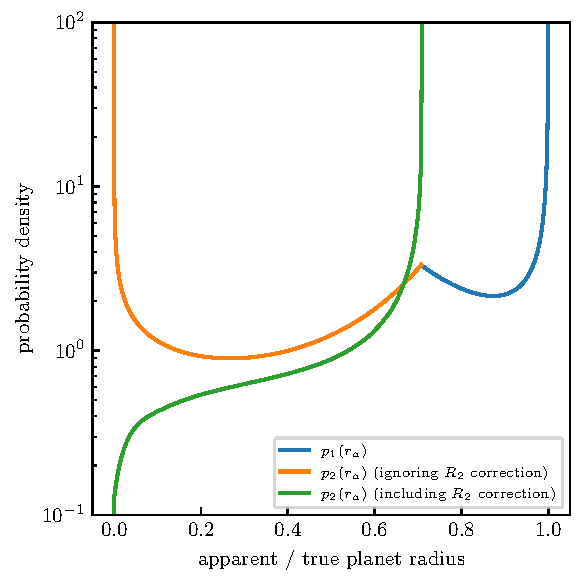
\includegraphics[width=.9\textwidth]{figures/prob_r_a.pdf}
    \end{center}
    \caption{Model \#2 (Sec.~\ref{sec:model_2}): 
    probability of observing an apparent radius $r_a$ given a 
    planet orbiting the primary, $p_1(r_a)$, or the secondary, $p_2(r_a)$ of a 
    binary system.
    The true planet radius is fixed~--~a delta function centered on ``1''.
    This plot takes $\alpha=3.5, \beta=0$, for $\alpha$ the exponent in 
    the mass-luminosity relation $L \propto M^\alpha$, and $\beta$ the 
    exponent in the distribution of mass ratios in a volume-limited sample.
    Each distribution is separately normalized.
    }
    \label{fig:model2_prob_r_a}
\end{figure}
